\chapter{Einführung Performanceanalyse}
\section{Motivation}

Die Performance respektive Leistungsfähigkeit einer Applikation stellt einer der bedeutendsten Qualitätsanforderungen dar. Sie kann nicht nur zu verärgerten Benutzern, sondern auch zu einer Verlangsamung der Business-Prozesse führen. Die Motivation für eine Performanceanalyse entsteht, wenn die in Service Level Agreement oder Anforderungsanalyse spezifizierten \textbf{Qualitätsanforderungen nicht erfüllt} sind. Optimal wäre, wenn diese Anforderung während des Entwicklungsprozesses kontinuierlich geprüft würden.

\section{Ablauf}
Die Performanceanalyse ist ein iterativer Prozess und sollte so lange dauern, bis die Anforderungen erfüllt und der Kunde zufrieden ist. Sie besteht aus folgenden vier Schritten\cite{hummelBeer201109}:
\begin{enumerate}
	\item Identifikation der neuralgischen Punkte des Systems
	\item \textbf{Suche nach dem Dominating Consumer\footnote{Kirk Pepperdine bezeichnet die Aktivität, welche dominiert wie die CPU gebraucht wird, als Dominating Consumer . } (siehe Abschnitt \ref{dominating_consumer})}
	\item \textbf{Sammeln von Detaildaten (siehe Abschnitt \ref{garbage_collection_tuning})}
	\item Lösen des Problems
\end{enumerate}


Damit die Analyse der Garbage Collection zum richtigen Zeitpunkt gemacht wird, sind insbesondere die Punkte zwei und drei wichtig. Sie werden in den folgenden beiden Abschnitten genauer definiert.
\section{Suche nach dem Dominating Consumer}\label{dominating_consumer}
Die Suche nach dem Dominating Consumer kann nach folgendem Schema durchgeführt werden:
\begin{figure}[H]
  	\centering
    	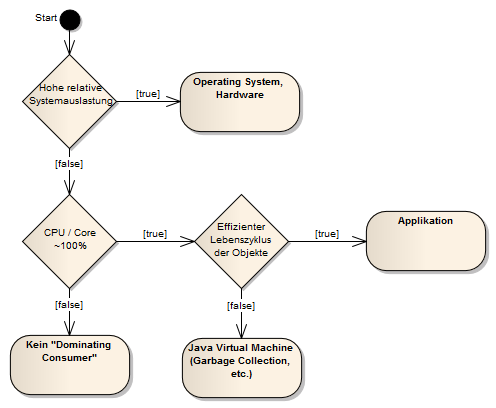
\includegraphics[width=13.1cm]{images/dominating_consumer}
        	\caption{Suche nach dem Dominating Consumer}
\end{figure}

\subsection{Hohe relative Systemlast}\label{hohe_systemauslastung}
Die erste Frage, die sich bei der Suche nach dem Dominating Consumer stellt, ist, ob die hohe CPU-Auslastung durch die Applikation oder das System verursacht wird. Je nach Betriebssystemen gibt es dafür unterschiedliche Werkzeuge:
\begin{itemize}
	\item Unter \textbf{Windows} kann dafür der \textit{Task Manager} verwendet werden. Auf der Lasche Performance müssen dafür allerdings auch die Kernelzeiten eingeschaltet werden.
	\item Unter \textbf{Linux respektive Unix} kann dafür das Programm \textit{vmstat} verwendet werden.
\end{itemize}

Hohe Systemauslastung kann unterschiedliche Gründe haben: 
\begin{itemize}
\item \textbf{Exzessive Kontextwechsel:} Mehrere Prozesse können sich die gleiche CPU (CPU-Kern) nur deshalb teilen, weil beim Wechsel von Prozess A auf B ein Kontextwechsel gemacht wird, so dass Thread B am selben Ort weiterarbeitet wo er beim letzten Mal war. Gründe für exzessives Kontextwechsel können beispielsweise nicht adäquat gewählte Locks sein. Wenn ein Thread aufgrund der Synchronisation angehalten werden muss.\footnote{Symptomatisch zeigt dann vmstat, das System ist nicht im Leerlauf, aber die Kernelzeiten (cpu/sy) dominieren die Zeit des Benutzers (cpu/us).}
\item \textbf{Viel Interaktion (Input/Output) mit der Festplatte} 
\item \textbf{Viel Interaktion mit dem Netzwerk} 
\end{itemize}


\subsection{Hohe CPU- respektive Core-Last}
Sofern die im Abschnitt \ref{hohe_systemauslastung} beschriebenen Punkte nicht zutreffen, stellt sich die Frage, ob die Auslastung der CPU überhaupt gross ist. Ist das nicht der Fall, gibt es womöglich keinen Dominating Consumer - es muss dann herausgefunden werden, was die Threads daran hindert, CPU Ressourcen zu verwenden. Es gibt dafür laut \cite{pepperdine201102} unterschiedliche Gründe:
\begin{itemize}
\item \textbf{Dead Locks: } Threads schliessen sich gegenseitig aus. Das würde man in einem Thread Dump (Stacktrace) anhand der vielen wartenden Threads erkennen. 
\item \textbf{Applikation skaliert nicht: } Applikation hat schlechte multi-core Eigenschaften. Das ist beispielsweise der Fall, wenn durch Synchronisation oder Memory Barrieren Engpässe entstehen - auch zu erkennen an wartenden Threads im Thread Dump.
\item \textbf{Langsame Disks / Netzwerke: }In einem Sampling oder Profiling wäre beispielsweise erkennbar, dass Threads oft in \textit{read}-Operationen stecken.
\item \textbf{Zu kleine Connection- und Thread-Pools}
\item \textbf{Aurufe auf langsame externe Systeme}
\end{itemize}


\subsection{Effizienter Objekt-Lebenszyklus}
Sofern die CPU-Auslastung, trotz kleiner relativer Systemlast durch die Applikation, hoch ist, muss unter anderem\footnote{auch der Optimizer könnte dafür verantwortlich sein} die Garbage Collection angeschaut werden. Dafür gibt es unterschiedliche Herangehensweisen:
\begin{itemize}
\item \textbf{Memory Analyse (Objektpopulation): }Es wird angeschaut, wie alt die Objekte in den unterschiedlichen Bereichen (Young Generation, Old Generation) sind. Wieviele Garbage Collection Zyklen sie überlebt haben.
\item \textbf{Garbage Collection: }Wann und wie oft werden Garbage Collections durchgeführt, wie lange haben sie gedauert, wieviel Speicher haben sie befreit.
\end{itemize}
Im weiteren konzentrieren wir uns auf die Ziele und Vorgehensweise beim Garbage Collection Tuning.

\section{Garbage Collection Tuning}\label{garbage_collection_tuning}
Mit dem Resultat der Analyse des Dominating Consumers entscheidet sich auch, in welchem Bereich weitere Detaildaten gesammelt werden müssen. Wir beschränken uns in diesem Abschnitt auf die Analyse im Bereich der Garbage Collection. Hier gilt grundsätzlich auch: "Never change a running system". Man ändert also nur etwas, wenn die Leistung den Anforderungen nicht genügt. 

In der Regel will man mit dem Tuning eines der drei unten stehenden Zielen erreichen\cite{langerkreftJavaCore}: 
\begin{itemize}
\item Verbesserung des Durchsatzes (siehe Abschnitt \ref{gc_tuning_durchsatz})
\item Geringere Pausenzeiten (siehe Abschnitt \ref{gc_tuning_pausenzeiten})
\item Geringerer Speicherverbrauch (siehe Abschnitt \ref{gc_tuning_speicherverbrauch})
\end{itemize}

Diese drei Ziele bilden eine Dreiecksbeziehung, zum Beispiel führt eine aggressive Optimierung des Durchsatzes in der Regel zu längeren Stop-the-World\footnote{Zeiten in welchen die Prozessoren der Anwendung keine Rechenzeiten zur Verfügung stellen.} Pausen. Tuning bedeutet nun, zwei der Ziele konstant zu halten, während das dritte durch Anpassung der Konfiguration verbessert wird. Sofern die Optimierung nicht ausreicht, muss einer der beiden anderen Parameter aufgegeben werden, um das Ziel zu erreichen.


\subsection{Durchsatz\label{gc_tuning_durchsatz}}
Die relative Zeit der CPU, welche der Anwendung zur Verfügung steht, nennt man Durchsatz (englisch \textit{Throughput}). Es handelt sich also um einen Prozentsatz im Vergleich mit der gesamten CPU-Zeit. Der Durchsatz wird folgendermassen berechnet:

 \begin{align*}
         Durchsatz &= 100 * (1-Relative\;Zeit\;in\;Garbage\;Collection)\\
         Durchsatz &= 100 * (1-\frac{Zeit\;in\;Garbage\;Collection}{Gesamtdauer\;der\;Messung})
 \end{align*}
Die Formel ist nur eine Annäherung und berücksichtigt weder nebenläufige Garbage Collection noch Maschinen mit mehreren Prozessorkernen, Durchsatz-Tuning spielt aber in der Praxis auch oft nur eine sehr untergeordnete Rolle\cite{langerkreftJavaCore}. Eine wirkliche Steigerung des Durchsatzes kann man nämlich nur mit einer aggressiven Optimierung erzielen, und die führt zu verlängerten Pausenzeiten, was nur bei Batch-Applikationen toleriert werden kann. Der Austausch der CPU oder das Zuschalten von weiteren ist normalerweise der kostengünstigere Weg.

\subsection{Pausenzeiten\label{gc_tuning_pausenzeiten}}
In der Regel geht es beim Garbage Collection Tuning um das Tuning der Pausenzeiten, dies weil man die Symptome wie das Stottern einer Anwendung nicht tolerieren kann. 

Man startet dann mit der Analyse einzelner Garbage Collections und versucht die Gründe für zu häufige oder zu lange dauernde Collections zu finden. Zu häufige Initiierung einer Garbage Collection kann unterschiedliche Gründe haben:
\begin{itemize}
\item \textbf{Erreichen eines Schwellenwerts des Young- oder Old-Spaces: } Anpassung der Grösse des Young- / Old-Spaces, Vergrösserung des Heaps, etc.
\item \textbf{Heap hat maximale Grösse erreicht:} Anpassung der Heap-Grösse, Beseitigung von Memory Leaks, etc.
\item \textbf{Allokation von Objekten ist nicht möglich:} Vergrösserung des Young-Space, Beseitung der Fragmentierung, etc. 
\item \textbf{Von der Applikation initiiert (durch System.gc()):} Von der Applikation ausgelöste Garbage Collection Kommandos können mittels Aktivierung eines Flags ignoriert werden.
\end{itemize}



\subsection{Speicherverbrauch\label{gc_tuning_speicherverbrauch}}
Dieses Tuningziel verliert insofern an Relevanz, weil 64-Bit-JVMs bei grossen Applikationen schon sehr verbreitet sind und damit die Adressierung von mehr Speicher möglich ist. Mit 32-Bit Adressen kam man früher schon eher an die Grenze (ein Teil des adressierbaren Bereichs bei 32-Bit-Adressen von 4GB wird noch für das Betriebssystem verwendet). Eine Optimierung im Bereich des Speicherverbrauchs hat in der Regel nichts mit Garbage Collection Tuning zu tun, sondern ist eine Analyse der Objektpopulation im Bereich der Applikation.

